\documentclass[12pt,a4paper]{article}

\usepackage[utf8]{inputenc}
\usepackage[T1]{fontenc}
\usepackage{lmodern}
\usepackage[margin=1in]{geometry}
\usepackage{setspace}
\usepackage{graphicx}
\usepackage{booktabs}
\usepackage{tabularx}
\usepackage{array}
\usepackage{hyperref}
\usepackage{xcolor}
\usepackage{fancyhdr}
\usepackage{float}
\usepackage{amsmath}
\usepackage{tikz}

\usetikzlibrary{arrows.meta, positioning, shapes.geometric, fit, backgrounds, decorations.pathreplacing}

% Color Theme
\definecolor{primary}{RGB}{15, 68, 113}
\definecolor{secondary}{RGB}{43, 114, 175}
\definecolor{accent}{RGB}{208, 83, 30}
\definecolor{bglight}{RGB}{247, 250, 252}
\definecolor{linegray}{RGB}{210, 218, 226}

\hypersetup{
    colorlinks=true,
    linkcolor=primary,
    urlcolor=secondary,
    pdftitle={CreditSense Professional Project Report},
    pdfauthor={Team CreditSense}
}

% Formatting
\setstretch{1.15}
\setlength{\parskip}{0.55em}
\setlength{\parindent}{0em}

% Header and Footer
\pagestyle{fancy}
\fancyhf{}
\lhead{\textcolor{gray}{\small CreditSense Professional Report}}
\rhead{\textcolor{gray}{\small Final Submission}}
\cfoot{\thepage}
\setlength{\headheight}{14.5pt}

\newcommand{\infobox}[2]{
    \vspace{0.2em}
    \noindent\fcolorbox{linegray}{bglight}{
        \begin{minipage}{0.965\linewidth}
        {\color{primary}\textbf{#1}}\\[0.35em]
        #2
        \end{minipage}
    }
    \vspace{0.3em}
}

\begin{document}

% ------------------------- TITLE PAGE ------------------------- %
\begin{titlepage}
    \centering
    \vspace*{2.0cm}

    {\Huge \bfseries \color{primary} CreditSense}\\[1.1cm]
    {\LARGE \bfseries AI-Assisted Credit Risk Assessment\\Platform}\\[1.7cm]

    {\Large \textit{A Project Report}}\\[0.7cm]
    {\Large \textit{Submitted by}}\\[1.0cm]

    \renewcommand{\arraystretch}{1.35}
    \begin{tabular}{ll}
        \textbf{Mitul Bhatia} & 2401010279 \\
        \textbf{Vaibhav} & 2401010486 \\
        \textbf{Sarvjeet} & 2401010424 \\
        \textbf{Hardik} & 2401010174 \\
    \end{tabular}

    \vfill
\end{titlepage}

\tableofcontents
\newpage

% ------------------------- ABSTRACT ------------------------- %
\section*{Abstract}
\addcontentsline{toc}{section}{Abstract}

CreditSense addresses a core fintech challenge: producing fast credit decisions without sacrificing regulatory compliance or explainability. Traditional underwriting is slow and manual, while unconstrained LLM systems can hallucinate policy logic and create audit risk.

This project implements a modular multi-agent architecture using LangGraph, FastAPI, Streamlit, deterministic policy computation, and Chroma-based retrieval with ONNX embeddings. The system combines conversational intake, regulatory context retrieval, explicit numeric risk scoring, and bilingual report generation in one controlled pipeline.

The resulting platform is submission-ready, operationally clear, and structured for practical deployment on constrained infrastructure.

% ---------------------- 1. EXECUTIVE SUMMARY ------------------ %
\section{Executive Summary}

\infobox{Problem Statement}{
Financial institutions need explainable and reproducible loan-assessment workflows. Purely manual processes are slow, and purely generative systems can violate compliance expectations.
}

\infobox{Project Objective}{
Design and implement a professional-grade, auditable underwriting assistant that provides deterministic decision support with context-grounded AI reporting.
}

\infobox{Delivered Outcome}{
An end-to-end platform with user intake, regulatory retrieval, policy evaluation, bilingual reporting, PDF export, and production-oriented repository operations including Git LFS for large artifacts.
}

% -------------------- 2. SYSTEM OVERVIEW ---------------------- %
\section{System Overview}

\subsection{Technology Stack}
\begin{tabularx}{\textwidth}{>{\bfseries}p{0.32\textwidth}X}
\toprule
Frontend & Streamlit conversational interface with structured borrower intake and report rendering \\
Backend API & FastAPI service layer for ingestion, chat orchestration, and report endpoints \\
Orchestration & LangGraph stateful agent routing across guardrail, intake, retrieval, policy, and reporting nodes \\
Retrieval & Chroma persistent store with ONNXMiniLM\_L6\_V2 embeddings \\
Decision Core & Deterministic policy engine and heuristic risk scorer \\
Report Output & English and Hindi narratives with PDF export workflow \\
\bottomrule
\end{tabularx}

\subsection{Why the Architecture is Professional}
\begin{itemize}
    \item Separation of concerns between interface, API orchestration, retrieval, scoring, and presentation.
    \item Deterministic numerical decision path for auditability.
    \item Controlled LLM usage for extraction and narrative generation, not final policy authority.
    \item Deployment-aware design for free-tier and low-resource environments.
\end{itemize}

% -------------------- 3. ARCHITECTURE ------------------------- %
\section{System Architecture and Data Flow}

\subsection{Architecture Diagram}
\begin{figure}[H]
\centering
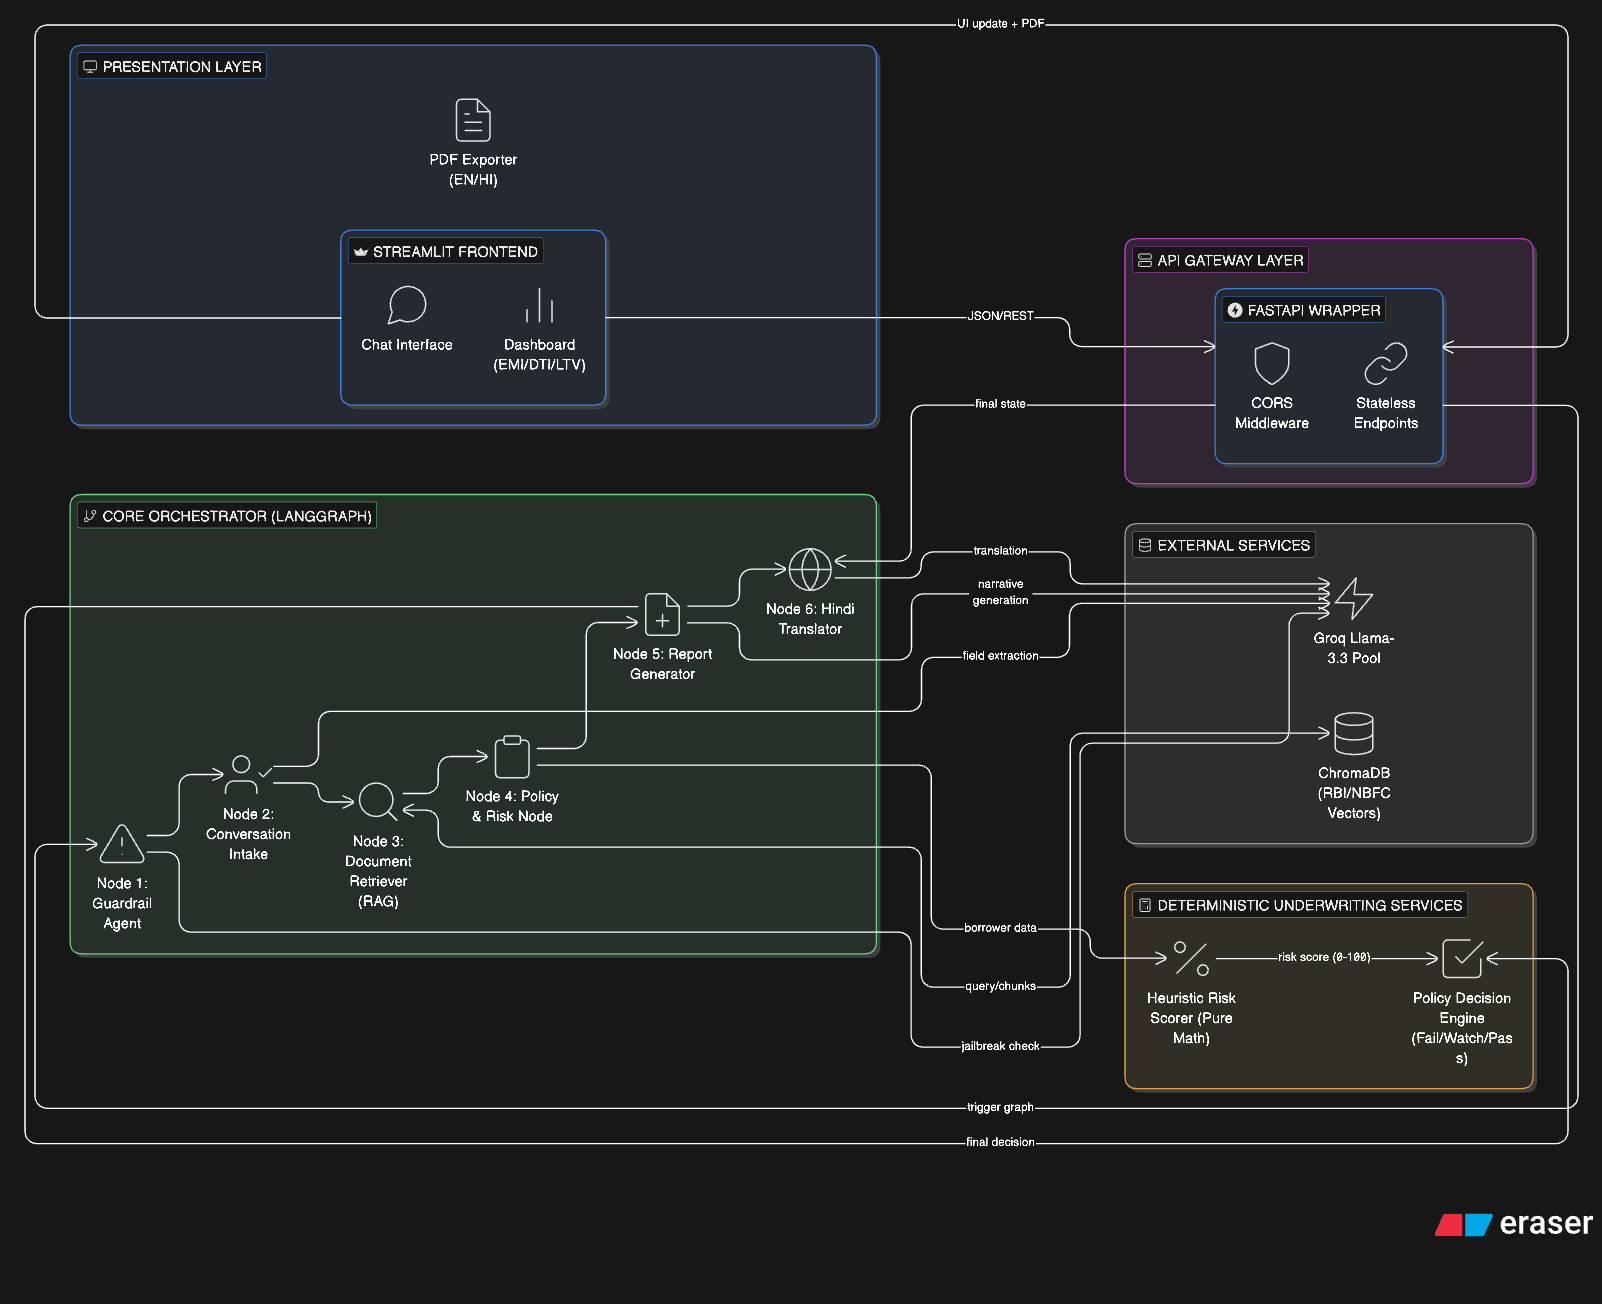
\includegraphics[width=\textwidth]{arhctecture_diagram.png}
\caption{CreditSense tri-layer architecture used for final submission}
\label{fig:creditsense-architecture}
\end{figure}

\subsection{Flow Interpretation by Layer}
\begin{tabularx}{\textwidth}{>{\bfseries}p{0.26\textwidth}X}
\toprule
Presentation Layer & User interaction, profile capture, and report delivery through Streamlit and PDF exporter \\
API Gateway Layer & Stateless request handling, schema enforcement, and controlled route execution \\
Core Orchestrator & Multi-agent graph with explicit state transitions across intake, retrieval, policy, and translation \\
External Services & LLM pool and Chroma retrieval backend for regulatory grounding \\
Deterministic Services & Risk scoring and final decision logic using transparent mathematical rules \\
\bottomrule
\end{tabularx}

\subsection{ONNX Migration Impact}
Early versions relying on full sentence-transformers and PyTorch introduced high memory pressure in constrained environments. The migration to ONNXMiniLM\_L6\_V2 through Chroma maintained semantic retrieval quality while significantly reducing runtime footprint and startup overhead.

% -------------------- 4. IMPLEMENTATION ----------------------- %
\section{Implementation Modules}

\begin{tabularx}{\textwidth}{>{\bfseries}p{0.24\textwidth} >{\bfseries}p{0.21\textwidth} X}
\toprule
Module & Layer & Responsibility \\
\midrule
Guardrail Agent & Orchestrator & Filters unsafe or irrelevant prompts before business processing \\
Conversation Intake & Orchestrator & Extracts borrower profile fields from natural language turns \\
Retriever Service & Retrieval & Queries Chroma collection and builds citation-ready context chunks \\
Policy Engine & Deterministic Logic & Computes DTI/LTV-driven outcomes and rules-based classification \\
Risk Scorer & Deterministic Logic & Produces transparent weighted risk score from borrower attributes \\
Report Generator & Reporting & Converts numeric outcomes into structured human-readable decision rationale \\
Translation Node & Reporting & Produces Hindi-compatible output for multilingual accessibility \\
PDF Exporter & Delivery & Generates downloadable final reports for submission and operations \\
\bottomrule
\end{tabularx}

% -------------------- 5. CONTRIBUTION MATRIX ------------------ %
\section{Contribution Matrix}

This matrix formalizes team ownership and deliverables for assessment and viva review.

\renewcommand{\arraystretch}{1.45}
\begin{tabularx}{\textwidth}{>{\bfseries}p{0.14\textwidth}>{\bfseries}p{0.25\textwidth}X}
\toprule
Member & Primary Ownership & Key Deliverables \\
\midrule
Mitul & Project Lead and Full-Stack Development & End-to-end architecture design, FastAPI backend, Streamlit integration, LangGraph orchestration, retrieval-service wiring, deployment flow, and final technical integration. \\
Vaibhav & Technical Documentation and Report Strategy & Structured technical documentation set, architecture write-ups, submission report curation, and narrative consistency across deliverables. \\
Sarvjeet & Media and Presentation Lead & Visual communication assets, final presentation deck, system-flow translation for audience-friendly explanation, and demo walkthrough packaging. \\
Hardik & Product Ideation and Strategy & Problem framing, requirements articulation, policy-threshold framing guidance, and solution direction aligned with practical user adoption. \\
\bottomrule
\end{tabularx}

% -------------------- 6. GIT LFS SECTION ---------------------- %
\section{Git LFS and Artifact Management}

\subsection{Why Git LFS Was Required}
This project contains large binary artifacts, especially vector-store database files used by Chroma. Standard Git is inefficient for large mutable binaries and can fail or bloat repository history when these artifacts are versioned directly.

\subsection{Project LFS Strategy}
\begin{itemize}
    \item Canonical milestone path normalized to \texttt{MILESTONE\_2/}.
    \item Large vector-store artifacts tracked with Git LFS under \texttt{MILESTONE\_2/creditsense/chroma\_store/}.
    \item Duplicate accidental path with spaces was removed to avoid dual database stores.
\end{itemize}

\subsection{Operational Workflow Used}
\begin{verbatim}
brew install git-lfs
git lfs install
git add .gitattributes
cd MILESTONE_2/creditsense/chroma_store
git add chroma.sqlite3
git commit -m "Track Chroma store with Git LFS"
git push origin main
\end{verbatim}

\subsection{Result}
Repository operations remained stable while retaining required large project assets for reproducible demonstrations and submission packaging.

% -------------------- 7. VALIDATION --------------------------- %
\section{Validation and Submission Readiness}

\begin{tabularx}{\textwidth}{>{\bfseries}p{0.30\textwidth}X}
\toprule
Validation Item & Outcome \\
\midrule
Architecture Included & Embedded directly in this report from the official project diagram asset \\
Contribution Matrix & Included as a formal table with role ownership and deliverables \\
Modular Report Structure & Organized into executive summary, architecture, modules, matrix, LFS, and readiness sections \\
Professional Formatting & Consistent typography, color hierarchy, tabular summaries, and structured section flow \\
PDF Generation Ready & TeX source organized for reproducible PDF build and final submission export \\
\bottomrule
\end{tabularx}

% -------------------- 8. CONCLUSION --------------------------- %
\section{Conclusion and Forward Path}

CreditSense demonstrates a practical, auditable, and presentation-grade approach to AI-assisted underwriting. The system balances deterministic policy enforcement with contextual AI capabilities, while repository operations were hardened through Git LFS for large data assets.

Immediate future enhancements include:
\begin{itemize}
    \item stronger authentication and role-based access controls,
    \item deeper monitoring and evaluation instrumentation,
    \item expanded benchmarking with larger historical credit datasets,
    \item automated CI checks for report and docs validation.
\end{itemize}

\end{document}
